\documentclass[../main.tex]{subfiles}
\graphicspath{{{chapter-continuous/img/}}{img/}}
\begin{document}
Continuous games are multiplayer games in which strategy sets are compact and utility functions are continuous. Many application domains have a~continuum of actions, such as the allocation of time, resources, location in space \cite{Kamra18}, or parameters of classifiers \cite{Loiseau19}. This also includes several games modeling cybersecurity scenarios \cite{Niu2021,Loiseau19,roussillon2021scalable}.

Continuous games have equilibria in mixed strategies by Glicksberg's generalization of Nash's theorem \cite{Glicksberg52}, but these equilibria are typically very hard to characterize and compute. We point out the main difficulties in the development of algorithms and numerical methods for continuous games:
\begin{itemize}
  \item The equilibrium can be any tuple of mixed strategies with infinite supports~\cite{Karlin59} or almost any tuple of~finitely-supported mixed strategies \cite{Rehbeck18}.
  \item Bounds on the size of supports of equilibrium strategies are known only for particular classes of continuous games \cite{stein.ozdaglar.ea:separable}.
  \item Some important games have only mixed equilibria; for example, certain variants of Colonel Blotto games \cite{Golman2009}.
  \item Finding a mixed strategy equilibrium involves locating its support, which lies inside a continuum of points.
\end{itemize}

To the best of our knowledge, algorithms and numerical methods exist only for very special classes of continuous games. In particular, two-player zero-sum polynomial games can be solved using sum-of-squares optimization based on a sequence of semidefinite relaxations of the original problem \cite{parrilo:polynomial,LarakiLasserre12}. \textcite{BasarOlsder99} have written a detailed analysis of equilibria for some families of games with a particular shape of utility functions (e.g., games of timing, bell-shaped kernels). Fictitious play, one of the principal learning methods for finite games, was recently extended to continuous action spaces and applied to Blotto games~\cite{Ganzfried21}. The dynamics of fictitious play have been analyzed only under further restrictive assumptions in the continuous setting \cite{Hofbauer06}. No-regret learning, studied by \textcite{Mertikopoulos2019}, can be applied to finding pure equilibria or to mixed strategy learning in finite games. Convergence guarantees for algorithms in the distributed environment solving convex-concave games and some generalizations thereof have been developed by \textcite{mertikopoulos.lecouat.ea:optimistic}. In a similar setting, \textcite{chasnov.ratliff.ea:convergence} provides convergence guarantees to a neighborhood of a stable Nash equilibrium for gradient-based learning algorithms.


\section{Basic Notions}
The player set is denoted by $N=\{1,\dots,n\}$. Each player $i\in N$ selects a pure strategy $x_i$ from a nonempty compact set $X_i\subseteq \R^{d_i}$, where $d_i$ is a positive integer. A~pure strategy profile is the $n$-tuple $\bx=(x_1,\dots,x_n)\in \bX$, where $\bX=X_1\times\dots\times X_n$. We assume that each utility function $u_i\colon \bX\to \R$ is continuous. A \emph{continuous game} is the tuple
\[
	\calG=\langle N,(X_i)_{i\in N},(u_i)_{i\in N}\rangle.
\]

A mixed strategy of player $i$ can be an arbitrary Borel probability measure $\mu_i$ over $X_i$. Note that this general framework allows us to consider mixed strategies whose support is uncountably infinite, which is inevitable for the coherent treatment of games over compact strategy sets.

By $M_i$ we denote the space of all mixed strategies of player $i\in N$. Let $\bM=M_1\times \dots \times M_n$ and let $\bmu=(\mu_1,\dots,\mu_n) \in \bM$ be a profile of mixed strategies. For the sake of brevity, we use $\bmu$ in place of the corresponding product probability measure $\mu_1\times\dots\times \mu_n$ in the definitions below involving integrals. The expected utility of player $i\in N$ is the function $U_i\colon \bM\to \R$
\[
    U_i(\bmu) =  \int_{\bX} u_i \dif\bmu
\]
This definition yields a function $U_i\colon \bM\to \R,$ which can be effectively evaluated only in special cases, such as when the support of each $\mu_i$ is finite.

We define the sets which exclude one player as
\[
\bX_{-i}=\bigtimes_{\substack{j\in N \\ j\neq i}} X_j \quad \text{and} \quad \bM_{-i}=\bigtimes_{\substack{j\in N \\ j\neq i}}M_j.
\]
For every $\bmu\in \bM$ and each player $i\in N$, by $\bmu_{-i}$ we denote the restriction of $\bmu$ onto $\bM_{-i}$.  The value of expected utility of player $i$ in a strategy profile $(x_i,\bmu_{-i})\in X_i\times \bM_{-i}$ is denoted by
\begin{equation}\label{def:EU}
    U_i(x_i,\bmu_{-i})=\int_{\bX_{-i}} u_i(x_i,.)\; \dif\bmu_{-i}.
\end{equation}

\begin{definition}[\textcite{Nash51}]\label{def:ne}
    A Nash equilibrium is a strategy profile $\bmu^\star\in\bM$ satisfying
    \begin{equation*}
        U_i(\bmu^\star)=\max_{x_i\in X_i} U_i(x_i,\bmu_{-i}^\star), \qquad \forall i\in N.
    \end{equation*}
    That is, each player's strategy is a best response against those of the others.
\end{definition}

\begin{theorem}[\textcite{Glicksberg52}]\label{thm:Glick}
    Every continuous game has a mixed strategy Nash equilibrium.
\end{theorem}

\section{Equilibria in Separable Network Games}
Separable network games \cite{Bregman98,Cai16} are multiplayer strategic games in which players interact only with adjacent players in a simple undirected graph. The utility of each player results from the aggregation of utilities in the corresponding general-sum two-player games. We extend this model to infinite \emph{network games} whose strategy sets are compact subsets of the Euclidean space. We show that \emph{Nash Equilibria} (NE) of a zero-sum continuous network game can be characterized as optimal solutions to a~specific infinite-dimensional linear optimization problem. In particular, when the utility functions are multivariate polynomials, this optimization formulation enables us to approximate the equilibria using a~hierarchy of semidefinite relaxations based on the Moment-SOS hierarchies discussed in \cref{sec:momsos}.
\subsection{Continuous Network Games}\label{sec:net}
Separable network games can capture situations in which players distribute their capacities or resources in a continuous way across multiple targets to achieve control over them. The targets can be battlefields, inspection sites, exit points etc.

In the class of games considered in this chapter, each player $i \in N$ is identified with a node of an undirected graph $(N,E)$ without loops. The presence of an edge $\{i,j\}\in E$ means that players $i$ and $j$ engage in a two-person general-sum strategic game in which the utility functions of players $i$ and $j$ are functions $u_{ij}\colon X_i\times X_j\to\R$ and $u_{ji}\colon X_j\times X_i\to\R$.

We will always assume that the functions $u_{ij}$ and $u_{ji}$ are at least integrable, ensuring that every expected utility appearing below is correctly defined. Typically, a player $i$ participates in multiple pairwise games, in which case, the same strategy strategy $x_i\in X_i$ is implemented in all two-person games played with the adjacent players in the graph $(N,E)$. Thus, the aggregated utility of player $i$ is computed as
\begin{equation}\label{def:pi}
    u_i(\bx) = \sum_{\substack{j\in N \\ \{i,j\}\in E}} u_{ij}(x_i,x_j), \qquad \bx\in\bX.
\end{equation}
The resulting $n$-person game with compact strategy sets is called a \emph{separable network game}, or ``network game'' for short. We say that $\calG$ is
\begin{itemize}
    \item a \emph{polymatrix game} when all strategy sets~$X_i$ are finite;
    \item \emph{zero-sum} if  $\sum_{i\in N} u_i(\bx)=0$ for all $\bx\in\bX$;
    \item \emph{continuous} if each utility function $u_i$ is continuous.
\end{itemize}
A class of network games often studied in the literature is the class of zero-sum polymatrix games. The ``global'' zero-sum assumption and finite strategy sets make such games computationally tractable \cite{Cai16,FPNet,Bailey19,Rubinstein,CaiDaskalkis}.

\begin{example}
Let $N=\{1,2,3,4\}$ and the graph $(N,E)$ be the cycle on \cref{fig:4}. This is the smallest example of a network game such that each player interacts only with a strict subset of other players. For example, the utility function of player $3$ is $u_3(x_1,x_2,x_3,x_4)=u_{31}(x_3,x_1)+u_{34}(x_3,x_4)$. The zero-sum condition for this game can be formulated as $u_3=-u_1-u_2-u_4$.
\end{example}

\begin{figure}[ht]
    \centering
  \begin{tikzpicture}
    \node[circle,fill=blue!20,draw,minimum size=0.5cm,inner sep=0pt] (1) {$1$};
    \node[circle,fill=blue!20,draw,minimum size=0.5cm,inner sep=0pt] (2) [right = 1cm  of 1]  {$2$};
    \node[circle,fill=blue!20,draw,minimum size=0.5cm,inner sep=0pt] (3) [below = 1cm  of 1] {$3$};
    \node[circle,fill=blue!20,draw,minimum size=0.5cm,inner sep=0pt] (4) [right = 1cm  of 3] {$4$};

    \path[draw,thick]
    (1) edge node {} (2)
    (1) edge node {} (3)
    (4) edge node {} (2)
    (3) edge node {} (4)
    ;
\end{tikzpicture}
    \caption{A network game with $4$ players and $4$ pairwise games}
    \label{fig:4}
\end{figure}

As a direct consequence of Glicksberg's theorem \ref{thm:Glick}, every continuous network game $\calG$ has a NE $\bmu^\star \in \bM$ in mixed strategies. We will show that the NE in a zero-sum continuous network game can be characterized using an optimization-based approach. Specifically, we consider the following infinite-dimensional linear optimization problem, which generalizes \emph{Linear Program 1} of \textcite{Cai16}:
\begin{mini!}{\bmu,\bw}{\sum_{i\in N} w_i} {\label{P}}{}
    \addConstraint{w_i}{\geq U_i(x_i,\bmu_{-i})\qquad \forall i\in N\enskip \forall x_i\in X_i} \label{P:ineq}
    \addConstraint{\bmu}{=(\mu_1,\dots,\mu_n) \in\bM}
    \addConstraint{\bw}{=(w_1,\dots,w_n) \in\R^n}
\end{mini!}

\begin{theorem}\label{thm:opti}
    For every profile of mixed strategies $\bmu^\star \in \bcalP$ in a zero-sum continuous network game $\calG$, the following are equivalent:
    \begin{enumerate}
        \item $\bmu^\star$ is a Nash equilibrium of game $\calG$.
        \item $(\bmu^\star, \bw^\star)$ is an optimal solution to (\ref{P}), where
        \begin{equation}\label{def:wi}
            w_i^\star = \max_{x_i \in X_i} U_i(x_i, \bmu_{-i}^\star), \qquad i \in N.
        \end{equation}
    \end{enumerate}
\end{theorem}

\begin{proof}
    Firstly, observe that the expression $\max_{\nu_i \in P_i} U_i(\nu_i, \bmu_{-i})$ is maximized by a $\nu_i$ supported on any of $U_i$'s maximizers. Therefore, given a feasible $(\bmu, \bw)$, the constraint (\ref{P:ineq}) implies
    \begin{equation}\label{ineq1}
        w_i \geq \max_{x_i \in X_i} U_i(x_i, \bmu_{-i}) = \max_{\nu_i \in P_i} U_i(\nu_i, \bmu_{-i}) \geq U_i(\mu_i, \bmu_{-i}) \quad \forall i \in N.
    \end{equation}
    Note that the maxima in inequalities (\ref{ineq1}) exist by compactness of $X_i$ and the continuity of the functions $U_i(\cdot, \bmu_{-i}) \colon X_i \to \R$. Applying inequalities (\ref{ineq1}) in the objective, together with the zero-sum property, gives:
    \begin{equation}\label{ineq3}
        \sum_{i \in N} w_i \geq \sum_{i \in N} U_i(\mu_i, \bmu_{-i}) = 0.
    \end{equation}

    By \cref{thm:Glick}, there exists an NE $\bmu^\star$ such that $U_i(\bmu^\star) = \max_{x_i \in X_i} U_i(x_i, \bmu_{-i}^\star) \; \forall i \in N$. Let $\bmu$ be an NE and $\bw^\star_i$ be as in condition (\ref{def:wi}), then the inequalities in (\ref{ineq1}) become equalities, and the lower bound of zero is achieved in (\ref{ineq3}).

    We have shown that NE correspond to optimal solutions. Conversely, consider any optimal solution $(\bmu^\star, \bw^\star)$. Notice that $w_i^\star$ must be tight upper bounds on $U_i(\cdot, \bmu_{-i}^\star)$. By the zero-sum property, $\sum_{i \in N} U_i(\bmu) = 0$ for any $\bmu$. If $\bmu^\star$ were not an NE, then there exists a player $i$ such that $\max_{x_i \in X_i} U_i(x_i, \bmu_{-i}) > U_i(\bmu)$. This implies that
    \[
        0 = \sum_{i \in N} U_i(\bmu) < \sum_{i \in N} \max_{x_i \in X_i} U_i(x_i, \bmu_{-i}) = \sum_{i \in N} w_i,
    \]
    i.e., the objective value is not optimal.
\end{proof}

The Borel probability measures and continuous functions in Problem~\ref{P} do not generally allow for effective computation. Still, there are cases where the solution can be computed. For example, in the case of zero-sum polymatrix games, Problem~\ref{P} becomes a linear program~\cite{Cai16}. Similarly, if we restrict the model to polynomial functions and semialgebraic sets, the solution can be computed using the tools of polynomial optimization discussed in \cref{sec:momsos}.
\subsection{Polynomial Network Games}\label{sec:poly}
In this section, we make the following assumptions about the strategy spaces and the utility functions of a network game $\calG$ defined by \eqref{def:game}.
\begin{enumerate}
    \item Every compact strategy space $X_i\subseteq \R^{m_i}$ is a \emph{basic semialgebraic set} $\calS(\bg_i)$ where each $g_{ik}$ is a real polynomial in $m_i$ variables and $K_i\neq\emptyset$ is a finite index set. We also assume the standard archimedean certificate of compactness  (\cref{def:archimedean}) on the sets.
    \item In every two-player game involving players $i,j\in N$, the utility functions $u_{ij}$ and $u_{ji}$ of player $i$ and $j$, respectively, are real polynomials in $m_i+m_j$ indeterminates.  Therefore, each utility function $u_i$ given by (\ref{def:pi}) is a real polynomial in $m_1+\dots + m_n$ indeterminates.
    \item The game $\calG$ is zero-sum.
\end{enumerate}
These three assumptions define a \emph{polynomial zero-sum network game} $\calG$. Glicksberg's theorem~(\ref{thm:Glick}) can be significantly strengthened for polynomial games --- each polynomial game has NE in which every player mixes only among finitely many pure strategies \cite{DresherKarlinShapley50,stein.ozdaglar.ea:separable}.

The solutions for polynomial zero-sum network games can be solved using Lasserre's hierarchies as described in \cref{sec:momsos}. Specifically, we relax the constraints on measures and polynomial inequalities of Program~\ref{P}. Instead of requiring that the mixed strategies of players lie in the cone of probability measures, we apply constraints on truncated sequences of moments. Similarly, we replace the inequalities \eqref{P:ineq} with the constraint that $w_i - U_i(\cdot, \bmu_{-i})$ lies in the truncated quadratic module.

The $h$-th level of the hierarchy is the following semidefinite program:
\begin{equation}
    \begin{aligned}
        \minimize_{\hat{\by}_1,\dots,\hat{\by}_n,\bw}\quad& w_1+\dots +w_n \\
        \text{\normalfont subject to}\quad
        & w_i - \bar{u}_i(\hat{\by}_{-i}) \in Q_{2h}(X_i) &\forall i \in N\\
        & \hat{\by}_i=(y_{i,\balpha})_{\balpha\in\N^{m_i}_{2h}} \text{ and $y_{i,\mathbf{0}}=1$} &\forall i \in N\\
        & M_h(\hat{\by}_i)\succeq 0 &\forall i \in N\\
        & M_h(g_{ik}, \hat{\by}_i)\succeq 0 & \forall k\in K_i,\, \forall i \in N\\
        & \bw=(w_1,\dots,w_n) \in\R^n \\
    \end{aligned}
    \label{momsdp}
\end{equation}

We then iteratively solve each level of the hierarchy until all sequences $\hat{\by}_i$ have a representing atomic measure, which we extract using the algorithm of \textcite[Algorithm 6.9]{Lasserre15:book}. With the strategies of other players fixed, the best response condition is equivalent to certifying optimality for a polynomial over a semialgebraic set.
\subsection{Experiments with Polynomial Network Games}
In the remaining part of this paper we show several examples of polynomial games and recovered their equilibria by the method explained in the \cref{sec:poly}. We implemented the hierarchy of programs \eqref{momsdp} in Julia using \href{https://jump.dev/}{JuMP} \cite{JuMP} and the \href{https://jump.dev/SumOfSquares.jl/stable/}{SumOfSquares.jl} package \cite{PolyJuMP}. We solved the semidefinite programs using \href{https://www.mosek.com/}{Mosek} on a laptop with a 3.1GHz dual-core CPU. Our code is available on GitHub at \href{https://github.com/votroto/PolyNets.jl}{https://github.com/votroto/PolyNets.jl}.

\begin{example}[Two-player zero-sum polynomial game]
    Consider a two-player zero-sum game with strategy sets $S_i$ given by
    \[
        S_{i} = \{ x \in \R \mid  -x^2 + 1 \ge 0 \}.
    \] 
    The utility functions are
    \[
        u_{1}(x_{1},x_{2}) = 2x_{1}x_{2}^2 - x_{1}^2 - x_{2} = -u_{2}(x_{1},x_{2}).
    \]
    Since polynomial network games are a generalization of polynomial games, we can use the same framework to solve them. A pure NE is achieved when Player 1 plays $x_{1} = 0.4$ and Player~2 plays $x_{2} = 0.63$. The optimal payoffs to each player are $\bw = (-0.47, 0.47)$. This problem was solved at order 4 of the hierarchy. Due to the low number of variables the problem required only 44 constraints and it was solved within 10\,ms.
\end{example}

\begin{example}[Three-player game with a complete graph]
    We consider a polynomial network game with the player set $N = \{1, 2, 3\}$. Each strategy set $S_i$ is equal to
    \[
        S_{i}   = \{ x \in \R \mid  -x^2 + 1 \ge 0 \}
    \]
    and the utility functions are
    \begin{equation*}\begin{aligned}
        u_{1}(x_{1},x_{2},x_{3}) &= -2x_{1}x_{2}^2 - 2x_{1}^2 + 5x_{1}x_{2} - 4x_{1}x_{3} - x_{2} - 2x_{3},\\
        u_{2}(x_{1},x_{2},x_{3}) &= 2x_{1}x_{2}^2 - 2x_{2}x_{3}^2 - 2x_{1}^2 - 5x_{1}x_{2} - 2x_{2}^2 + 5x_{2}x_{3} + x_{2},\\
        u_{3}(x_{1},x_{2},x_{3}) &= 2x_{2}x_{3}^2 + 4x_{1}^2 + 4x_{1}x_{3} + 2x_{2}^2 - 5x_{2}x_{3} + 2x_{3}.\\
    \end{aligned}\end{equation*}
    A partially mixed Nash equilibrium is this strategy profile:
        \[\begin{aligned}
        x_1 &= -0.06\\
        x_2 &= 0.35\\
        x_3 &=\begin{cases}
            1 &72\%\\
            -1 &28\%\\
        \end{cases}
    \end{aligned}\]
    The corresponding utilities are $\bw = (-1.22, 0.26, 0.97)$. This problem converged at order 4, resulting in 96 constraints. The solve time was around 10\,ms.
\end{example}

\begin{example}[Polynomial security game]
   We consider a polynomial security game with attackers $N_A=\{1,2\}$, defenders $N_D=\{3,4\}$, and targets $T_3=\{t_1,t_2\}$ and $T_4=\{t_3,t_4\}$. The capacities of attackers are $a_1=0.5$, $a_2=0.8$, and the defenders' capacities are $d_3=d_4=1$. The efficiency functions are:
    \begin{equation*}\begin{aligned}
        e_{t1}(x,y) &= (1-y^2)\cdot 0.7x^2\\
        e_{t2}(x,y) &= (y^2 -2y +1)\cdot (1.4x - 0.7x^2)\\
        e_{t3}(x,y) &= (1-y^2)\cdot (1.8x - 0.9x^2)\\
        e_{t4}(x,y) &= (y^2 -2y +1)\cdot 0.9x^2\\
    \end{aligned}\end{equation*}
    Our algorithm returns the partially mixed strategy profile at order 6:
    \[\begin{aligned}
        (x_{1,t_1}, x_{1,t_2}, x_{1,t_3}, x_{1,t_4}) &=
            (0.29, 0.0, 0.0, 0.21) \\
        (x_{2,t_1}, x_{2,t_2}, x_{2,t_3}, x_{2,t_4}) &=
            (0.36, 0.13, 0.04, 0.24) \\
        (y_{1,t_1}, y_{1,t_2}) &=\begin{cases}
            (0.33, 0.67) &46\%\\
            (0.69, 0.31) &54\%\\
        \end{cases}\\
        (y_{2,t_2}, y_{2,t_4}) &=\begin{cases}
            (0.46, 0.54) &2\%\\
            (0.08, 0.92) &6\%\\
            (0.91, 0.09) &92\%\\
        \end{cases}
    \end{aligned}\]
    The payoffs to each player are $\bw = (0.1, 0.3, -0.17, -0.23)$. While the payoffs converged at order 4 already and took only 3 seconds to solve, the corresponding strategies could only be extracted at order 6, which took 6 minutes to solve. Due to the high dimensionality of the utility functions and the fast growth of the hierarchy, the resulting SDP contained over 25 thousand constraints.
\end{example}

While running the experiments, we noticed the payoffs computed by this method are generally of high quality regardless of the solver used; The corresponding measures, on the other hand, were less accurate. For example, the strategy in the last example yields a loss of only $0.16$ instead of $0.17$. This appears to be a problem inherent to our approach rather than something that could be fine-tuned within the solvers.


\section{Approximate Equilibria in Generic Games}
\todo[inline]{combine with Quack. show the difference between specialized oracles and master-problems vs just logit and gurobi}
\todo[inline]{add results for all games}

In this section we present an algorithm that is much more widely applicable at the cost of relaxing the requirement on the exactness of solutions from the previous section. We focus on the computation and approximation of mixed strategy equilibria for the whole class of multiplayer general-sum continuous games. To solve such generic games, we vastly extend the scope of applicability of the double oracle algorithm, initially designed and proved to converge only for two-player zero-sum games. Specifically, we propose an iterative strategy generation technique, which splits the original problem into the master problem with only a finite subset of strategies being considered, and the subproblem in which an oracle finds the best response of each player. This simple method is guaranteed to recover an approximate equilibrium in finitely many iterations.

Further, we argue that the Wasserstein distance (the earth mover's distance) is the right metric for the space of mixed strategies for our purposes. Our main result is the convergence of this algorithm in the Wasserstein distance to an equilibrium of the original continuous game. The numerical experiments show the performance of our method on several classes of games including randomly generated examples.

The double oracle algorithm \cite{McMahan03} was extended from finite games and proved to converge for all two-player zero-sum continuous games \cite{Adam21}. The algorithm is relatively straightforward. It is based on the iterative solution of finite subgames and the subsequent extension of the current strategy sets with best response strategies. Despite its simplicity, this method was successfully adapted to large extensive-form games \cite{Bosansky14}, Bayesian games \cite{Li21}, and security domains with complex policy spaces \cite{Xu21}.

In this contribution, we extend the double oracle algorithm beyond two-player zero-sum continuous games \cite{Adam21}. This is a significant extension since we had to design a new convergence criterion to track the behavior of the algorithm. On top of that, there are relatively few methods for computing or approximating equilibria of continuous games, which narrows down the continuous games for which the exact solution can be found and used as a benchmark in our experiments. Our main result guarantees that the new method converges in the Wasserstein distance to an equilibrium for any general-sum $n$-player continuous game. Interestingly enough, it turns out that the Wasserstein distance represents a very natural metric on the space of mixed strategies. We demonstrate the computational performance of our method on selected examples of games appearing in the literature and on randomly generated games.
\subsection{Basic Notions}
Consider a game $\calG = \langle N,(X_i)_{i\in N},(u_i)_{i\in N}\rangle$ and nonempty compact subsets $Y_i\subseteq X_i$ for each player $i$ from the player set $N$. When each $u_i$ is restricted to $Y_1\times\dots\times Y_n$, the continuous game $\langle N,(Y_i)_{i\in N},(u_i)_{i\in N}\rangle$ is called the \emph{subgame} of~$\calG$.

The \emph{support} of a mixed strategy $\mu$ is the compact set defined by
\[
	\spt \mu = \bigcap \{K\subseteq X\mid K \text{ compact},\, \mu(K)=1\}.
\]

In this section, we will construct mixed strategies with finite supports. The support of Dirac measure $\delta_x$ is the singleton $\spt \delta_x=\{x\}$, where $x\in X_i$. In~general, when the support $\spt \mu$ of a mixed strategy $\mu$ is finite, it means that $\mu(x)>0$ for all $x\in \spt \mu$ and $\sum_{x\in \spt \mu} \mu(x)=1$. For clarity, we emphasize that a finitely-supported mixed strategy $\mu_i$ of player $i$ should be interpreted as the function $\mu\colon X_i\to [0,1]$ vanishing outside $\spt \mu_i$, and not as a vector of probabilities with a fixed dimension. This is because only the former viewpoint enables us to consider the distance between \emph{any} pair of pure strategies in $X_i$, which makes it possible to compute a distance between mixed strategies with \emph{arbitrary} supports.

For any $\eps\geq 0$, an \textit{$\epsilon$-equilibrium} is a mixed strategy profile $\bmu^\star\in \bM$ such that
\[
	U_i(x_i,\bmu_{-i}^\star) - U_i(\bmu^\star) \leq \eps, \qquad \text{for every $i\in N$ and $x_i\in X_i$.}
\]
This implies that for every $p_i\in \calM(X_i)$, the inequality $U_i(p_i,\bmu_{-i}^\star) - U_i(\bmu^\star) \leq \eps$ also holds.

We introduce the vector notation
\[
	\bU(\bmu) = (U_1(\bmu), \dots, U_n(\bmu)).
\]
Furthermore, we define
\[
	\bU(\bx,\bmu) = (U_1(x_1,\bmu_{-1}), \dots, U_n(x_n,\bmu_{-n})),
\]
for any $\bx\in\bX$ and $\bmu\in \bM$.

\begin{definition}
	Given an arbitrary positive parameter $\epsilon$, an $\epsilon$-equilibrium is a strategy profile $\bmu^\star\in \bM$ satisfying
	\[
		\bU(\bx,\bmu^\star) - \bU(\bmu^\star) \leq \beps, \qquad \forall \bx\in\bX,
	\]
	where $\beps$ is the vector $(\eps, \dots, \eps)$.
\end{definition}

\subsection{Convergence of Mixed Strategies}
We consider an arbitrary metric~$\rho_i$ on the compact strategy space $X_i\subseteq \R^{m_i}$ of each player $i\in N$. This enables us to quantify a~distance between pure strategies $x,y \in X_i$ by the number $\rho_i(x,y)\ge 0$. Consequently, we can define the Wasserstein distance $d_W$ on $\calM(X_i)$, which is compatible with the metric of the underlying strategy space $X_i$ in the sense that
\[
	d_W(\delta_x,\delta_y)=\rho_i(x,y),\qquad \forall x,y \in X_i.
\]
 The preservation of distance from $X_i$ to $\calM(X_i)$ is a very natural property, since the space of pure strategies $X_i$ is embedded in $\calM(X_i)$ via the correspondence $x\mapsto \delta_x$ mapping the pure strategy $x$ to the Dirac measure $\delta_x$.

The Wasserstein distance originated from optimal transport theory. It is nowadays highly instrumental in solving many problems of computer science. Specifically, the \emph{Wasserstein distance} of mixed strategies $p,q\in \calM(X_i)$ is
\[
	d_W(p,q) = \inf_{\mu} \int_{X_i^2} \rho_i(x,y) \dif\mu(x,y),
\]
where the infimum is over all Borel probability measures $\mu$ on $X_i^2$ whose one-dimensional marginals are $p$ and $q$:
\begin{align*}
  \mu(A\times X_i) & = p(A),\\
  \mu(X_i \times A)  & = q(A),
\end{align*}
for all Borel subsets $A\subseteq X_i$.

The dependence of $d_W$ on the metric $\rho_i$ is understood. The function $d_W$ is a metric on $\calM(X_i)$. Since $X_i$ is compact, it has necessarily bounded diameter. This implies that the convergence in $(\calM(X_i),d_W)$ coincides with the weak convergence \cite[Corollary 2.2.2]{Panaretos20}. Specifically, the following two assertions are equivalent for any sequence $(p^j)$ in $\calM(X_i)$:
\begin{enumerate}
  \item $(p^j)$ converges to $p$ in $(\calM(X_i),d_W)$.
  \item $(p^j)$ \emph{weakly converges} to $p$, which means by the definition that
\[
	\lim_{j} \int\nolimits_{X_i}f \dif p^j =  \int\nolimits_{X_i}f \dif p,
\]
for every continuous function $f\colon X_i\to \R$.
\end{enumerate}

The metric space $(\calM(X_i),d_W)$ is compact by \cite[Proposition 2.2.3]{Panaretos20}. Consequently, the joint strategy space $\bM$ is compact in a product metric as well, and any sequence $(\bmu^j)$ in $\bM$ has an accumulation point. Equivalently, the previous assertion can be formulated as follows.
\begin{proposition}\label{prop:convergence}
	Any sequence of mixed strategy profiles $(\bmu^j)$ in $\bM$ contains a~weakly convergent subsequence.
\end{proposition}

The function $U_i$ is continuous on $\bM$ by the definition of weak convergence. This implies that if $(\bmu^j)$ weakly converges to $\bmu$ in $\bM$, then the corresponding values of expected utility goes to $U_i(\bmu)$, that is, $\lim_j U_i(\bmu^j) = U_i(\bmu)$.
By compactness of~$\calM(X_i)$ and continuity of $U_i$, all maxima and maximizers appearing in the paper exist. This implies that the optimal value of utility function in response to the mixed strategies of other players is attained for some pure strategy. Proposition~\ref{prop:switch} is the precise formulation of this useful fact.

In the rest of this section, we will discuss the problem of computing and approximating the Wasserstein distance $d_W(p,q)$ of any pair of mixed strategies $p,q\in \calM(X_i)$ for player $i$. In general, this is a difficult infinite-dimensional optimization problem \cite{Peyre19}. In our setting it suffices to evaluate $d_W(p,q)$ only for mixed strategies with finite supports. In particular, it follows immediately from the definition of $d_W$ that
\[
	d_W(p,\delta_y)=\sum_{x\in \spt p}\rho_i(x,y)p(x),
\]
for every finitely-supported mixed strategy $p\in \calM(X_i)$ and any $y \in X_i$. If mixed strategies $p$ and $q$ have finite supports, then computing~$d_W(p,q)$ becomes the linear programming problem
\begin{equation}
	\label{def:LPobj}
	\begin{aligned}
	\min_{\mu(x,y)}\quad \sum_{x\in \spt p} \sum_{y\in \spt q} \rho_i(x,y) \mu&(x,y)\\
											\mu(x,y)  &\ge 0   &\forall (x,y)\in\spt p \times \spt q\\
		\sum_{x\in \spt p} \sum_{y\in \spt q}\mu(x,y)  &=1, \\
							\sum_{y\in \spt q}\mu(x,y) &= p(x)  &\quad \forall x\in \spt p \\
							\sum_{x\in \spt p}\mu(x,y) &= q(y)  &\quad \forall y\in \spt q
	\end{aligned}
\end{equation}
with variables $\mu(x,y)$ indexed by $(x,y)\in\spt p \times \spt q$.

\subsection{Main Results}
\input{chapter-continuous/oracle-results.tex}
\subsection{Implementation of the Master Problem}


Continuing with the established notation, let $w_i \in \R$ be the bound on player $i$'s utility, and let $\bmu$ be probability simplices defining the mixed strategies of players. The multilinear feasibility program in $\bw$ and $\bmu$ for finding NE in general-sum games is
\begin{equation}\label{eq:sturmfels}
	\begin{aligned}
		\sum_{i \in N} U_i(\bmu) &\ge \sum_{i \in N} w_i \\
		U_i(x, \bmu_{-i}) &\le w_i \quad &\forall i \in N, x \in X_i \\
		\sum_{x \in X_i} \mu_i(x) &= 1 \quad &\forall i \in N \\
		0 \le \mu_i(x) &\le 1 \quad &\forall i \in N, x \in X_i
	\end{aligned}	
\end{equation}

As the utility functions are defined by tensors and strategy spaces are finite, the definitions of expected utility simplify into weighted sums. Specifically, the best response function $U_i(x, \bmu_{-i})$ reduces to the vector
\[
	\sum_{\bx_{-i} \in \bX_{-i}} U_i[x,\bx_{-i}] \prod_{j \in N_{-i}} \mu_j[x_j];
\] while the expected utility $U_i(\bmu)$ becomes 
\[
	\sum_{\bx \in \bX} U_i[\bx] \prod_{i \in N} \mu_i[x_i].
\]

As mentioned in \cref{sec:sbab}, algebraic functions can be decomposed into binary operations for which there exist known tight convex relaxations. Specifically, the multilinear program \ref{eq:sturmfels} can be reformulated as a non-convex quadratically-constrained quadratic program, which can then be solved by spatial Branch and Bound solvers.

\todo[inline]{describe our choice and the advantages of each approach}



\begin{figure}
    \centering
    
\includegraphics[width=\textwidth]{general.runtimes.pdf}
    \caption{Runtime comparison between the bilinear formulation and the \emph{gambit-logit} algorithm on two-player general-sum matrix games with normally distributed payoffs. Each algorithm was executed 100 times per game size with a 20-second time limit. Mean runtimes of successful runs are overlaid as thick lines. Although the bilinear program exhibits lower median runtimes (shown as darkest plot regions) compared to \emph{gambit-logit} with default settings, its runtime has a multimodal distribution with a significantly higher standard deviation (5.15 s vs. 0.22 s for $30\times30$ games) leading to frequent timeouts. The \emph{gambit-logit} program always finished successfully, while the success rate of the bilinear formulation was steadily decreasing, completing 89\% of the 30-action games and only 59\% of 40-action games. Mean runtimes on 20-action games were: 0.81 s (bilinear) and 0.18 s (\emph{gambit-logit}).}
    \label{fig:general.runtimes}
\end{figure}

\begin{figure}
    \centering
    
\includegraphics[width=\textwidth]{testfun.runtimes.pdf}
    \caption{Runtime comparison between the bilinear formulation and the \emph{gambit-logit} algorithm on two-player general-sum matrix games. Each algorithm was executed 100 times per game size with a 20-second time limit. Solid lines represent mean runtimes. Payoff matrices were generated by evaluating the Michalewicz function for Player 1 and McCormick function for Player 2 on a Cartesian product of randomly sampled actions uniformly distributed over $[0, \pi]$. This test should provide a more realistic benchmark for the Double Oracle master-problem compared to normally-distributed random matrices.}
    \label{fig:testfun.runtimes}
\end{figure}

\begin{figure}
    \centering
    
\includegraphics[width=\textwidth]{zero.runtimes.pdf}
    \caption{Runtime comparison of the bilinear program, linear program, and the \emph{gambit-logit} algorithm for solving two-player zero-sum matrix games with normally distributed payoffs. Each algorithm was executed 100 times per game size with a 20-second time limit. Thick lines indicate mean runtimes of successful executions. For 20-action games, mean runtimes were: 0.6 ms (bilinear program), 0.02 ms (linear program), and 159.7 ms (\emph{gambit-logit}).}
    \label{fig:zero.runtimes}
\end{figure}

\subsection{Implementation of the Oracles}

In games with polynomial utility functions, the best response oracles can employ both methods of the methods of global optimization described in Chapter \ref{ch:global}. In the rest of the games we use the spatial Branch and Bound approach as the best response oracle. From our experience, local solvers can work sufficiently well as oracles in some games, although no convergence guarantees then apply. \todo[inline]{this belongs elsewhere (to the "this is a metaalgorithm parametrized by master and oracle...".... ok now it's here)}

blah...The examples in our collections have utilities specified in terms of sums and products of functions such as logarithms and square roots. All such functions should be accepted either directly by global solvers or through external modeling libraries such as \textsc{ampl}.
\todo[inline]{merge this properly}

We show a comparison of Oracle implementations based on non-linear solvers.
While we have succesfully used local-solvers as oracles, it is important to remember that convergence to equilibria is no longer guaranteed.
Regardless, we compare their performance in some of the following experiments.

The experiments are split into three groups, random polynomials, non-polynomial test functions, and a practical experiment
where we solve a where we run a fixed number of iterations of Double Oracle on the Colonel Blotto game.


\paragraph{polynomials}
blah

\paragraph{non-polynomial test functions}
blah

The next experiment is a measurement of the runtime of different solvers in practice over a course of ten iterations of double oracle in a game of General Blotto. The utility functions in \emph{General Blotto} games are sums of non-linearly weighted margins of victory over sets of fronts.
We chose a game with three isolated fronts defined by the utility $u_1(x_1, x_2) = \sum_{j=1}^m f\left( x_{1j} - x_{2j} \right)$ with a non-differentiable weighing function $f(z) = \operatorname{sgn}(z)\,|z|^{0.5}$. This game exhibits very slow convergence with the Double Oracle algorithm.
\iffalse
Multilinear terms, square roots and sums can be formulated directly via the generic modelling languages \emph{JuMP}, and \emph{AMPL}; however the sign function and absolute value are more challenging. Due to a lack of support and differentiability, all of the solvers: \emph{Ipopt}, \emph{Bonmin}, \emph{Couenne}, \emph{SCIP}, and \emph{Gurobi} were unable to solve a direct formulation of the oracle problem. Instead, we reformulated the weighing function $f$ using a binary variable as $f(x) = (2b-1)z$, subject to the constraints:
\[
\begin{aligned}
b &\in \{0,1\} \\
s,n,p &\in [0,1] \\
p &\leq b \\
n &\leq 1-b \\
x &= p - n \\
z^2 &=  p + n. \\
\end{aligned}
\]
The reformulation is a mixed-integer quadratic program.
\fi
\subsection{Numerical Experiments}\label{sec:custom.oracles}


We show the performance that can be expected from Multiple Oracle when using custom oracles on various important examples from the literature. In this section we present only the examples which we thought demonstrate interesting behaviors. In appendix \ref{appendix:do.results}, we follow with a more comprehensive evaluation of the algorithm using a generic master problem and oracles based on global optimization.

In some cases we show the progress of the convergence-criterion value \eqref{crit1} called ``instability'' over the course of $10$ iterations, and we also plot the Wasserstein distance \eqref{crit2} between mixed strategies in consecutive iterations. Each experiment was initialized with a randomly chosen feasible pure strategy. In games with polynomial utility functions, the best response oracles can employ both methods of the methods of global optimization described in Chapter \ref{ch:global}. In the rest of the games we use the spatial Branch and Bound approach as the best response oracle. From our experience, local solvers can work sufficiently well as oracles in some games.


\begin{example}[General Blotto]
    

The \emph{Double Oracle} algorithm converges unusually slowly (see Fig \ref{fig:ex.blotto.slow} for a game with 3 fronts) on the \emph{General Blotto} game valuing isolated fronts with $p=0.5$. Large gains are possible by winning a front by a small margin as the slope of the utility function around zero approaches infinity. After 40 iterations, the algorithm recovers the following $\epsilon$-NE with $\epsilon=0.03$:

\begin{figure}
\centering
\begin{tikzpicture}
\begin{groupplot}[
    group style={
        group size=2 by 1,
        horizontal sep=0.3cm
    },
    width=6cm,
    height=5cm,
    xlabel=Iteration,
    xmin=0,
    ymin=1e-6,
    xmax=41,
    ymode=log,
    legend style={
            at={(1.04,1.08)},
            anchor=south,
        legend columns=-1,
        column sep=1ex
    }
]

\pgfplotstableread{
0.41 0.41
0.29 0.29
0.29 0.35
0.24 0.1
0.22 0.51
0.18 0.068
0.11 0.25
0.12 0.17
0.091 0.15
0.1 0.11
0.094 0.11
0.18 0.085
0.14 0.11
0.1 0.13
0.12 0.076
0.069 0.11
0.074 0.078
0.071 0.091
0.043 0.049
0.061 0.045
0.043 0.046
0.046 0.046
0.045 0.062
0.045 0.031
0.054 0.038
0.024 0.053
0.043 0.048
0.06 0.054
0.054 0.058
0.047 0.039
0.033 0.039
0.038 0.028
0.032 0.025
0.038 0.02
0.03 0.029
0.029 0.023
0.019 0.026
0.027 0.025
0.029 0.023
0.021 0.032
}\exploitdata
\pgfplotstableread{
NaN NaN
1.2 1.2
0.6 0.87
0.44 0.41
0.71 0.81
0.65 0.57
0.42 0.22
0.33 0.21
0.21 0.18
0.18 0.15
0.14 0.17
0.17 0.17
0.16 0.27
0.14 0.21
0.12 0.15
0.14 0.14
0.14 0.17
0.11 0.11
0.1 0.098
0.16 0.11
0.17 0.11
0.13 0.074
0.12 0.062
0.11 0.054
0.048 0.073
0.1 0.078
0.082 0.083
0.091 0.097
0.071 0.079
0.096 0.06
0.083 0.069
0.089 0.092
0.06 0.07
0.034 0.083
0.063 0.064
0.06 0.087
0.062 0.09
0.044 0.047
0.056 0.046
0.074 0.049
}\wassersteindata

\pgfplotstablegetcolsof{\exploitdata}
\pgfmathtruncatemacro{\numcols}{\pgfplotsretval}

\nextgroupplot[ylabel=Exploitability]
\pgfplotsinvokeforeach{0,...,\numcols-1}{
    \addplot table[x expr=\coordindex+1, y index=#1] {\exploitdata};
}
\pgfplotsinvokeforeach{1,...,\numcols}{
    \addlegendentry{Player #1}
}

\nextgroupplot[ylabel=Wasserstein, ylabel near ticks, yticklabel pos=right]
\pgfplotsinvokeforeach{0,...,\numcols-1}{
    \addplot table[x expr=\coordindex+1, y index=#1] {\wassersteindata};
}

\end{groupplot}
\end{tikzpicture}
\caption{Slow convergence of a continuous but non-differentiable \emph{General Blotto} game valuing 3 isolated fronts with $p=0.5$. Both players can still profitably deviate by $0.02$ and $0.03$ utility units after 40 iterations. }
\label{fig:ex.blotto.slow}
\end{figure}

\begin{align*}
\mu_1^\star &\approx 0.003\delta_{ (0.15, 0.69, 0.16) } + 0.005\delta_{ (0.18, 0.16, 0.67) } + 0.006\delta_{ (0.57, 0.35, 0.08) } \\&+ 0.01\delta_{ (0.0, 0.5, 0.5) } + 0.011\delta_{ (0.45, 0.04, 0.51) } + 0.012\delta_{ (0.38, 0.11, 0.5) } \\&+ 0.018\delta_{ (0.09, 0.25, 0.66) } + 0.022\delta_{ (0.55, 0.01, 0.44) } + 0.026\delta_{ (0.06, 0.65, 0.29) } \\&+ 0.026\delta_{ (0.08, 0.52, 0.4) } + 0.029\delta_{ (0.49, 0.18, 0.32) } + 0.029\delta_{ (0.24, 0.16, 0.6) } \\&+ 0.032\delta_{ (0.44, 0.36, 0.2) } + 0.035\delta_{ (0.36, 0.0, 0.64) } + 0.039\delta_{ (0.04, 0.4, 0.55) } \\&+ 0.041\delta_{ (0.33, 0.12, 0.54) } + 0.041\delta_{ (0.28, 0.64, 0.08) } + 0.049\delta_{ (0.4, 0.02, 0.58) } \\&+ 0.051\delta_{ (0.2, 0.34, 0.46) } + 0.053\delta_{ (0.13, 0.55, 0.32) } + 0.061\delta_{ (0.26, 0.08, 0.66) } \\&+ 0.061\delta_{ (0.18, 0.58, 0.24) } + 0.069\delta_{ (0.0, 0.61, 0.39) } + 0.12\delta_{ (0.51, 0.45, 0.04) } \\&+ 0.151\delta_{ (0.64, 0.22, 0.14) },\\ 
\mu_2^\star &\approx 0.006\delta_{ (0.07, 0.66, 0.26) } + 0.009\delta_{ (0.0, 0.41, 0.59) } + 0.011\delta_{ (0.19, 0.59, 0.22) } \\&+ 0.012\delta_{ (0.54, 0.33, 0.13) } + 0.016\delta_{ (0.41, 0.14, 0.45) } + 0.02\delta_{ (0.0, 0.5, 0.5) } \\&+ 0.021\delta_{ (0.36, 0.4, 0.24) } + 0.023\delta_{ (0.44, 0.56, 0.0) } + 0.026\delta_{ (0.02, 0.61, 0.37) } \\&+ 0.028\delta_{ (0.14, 0.47, 0.39) } + 0.031\delta_{ (0.11, 0.26, 0.63) } + 0.033\delta_{ (0.37, 0.54, 0.09) } \\&+ 0.034\delta_{ (0.44, 0.51, 0.05) } + 0.037\delta_{ (0.5, 0.07, 0.43) } + 0.041\delta_{ (0.21, 0.32, 0.47) } \\&+ 0.045\delta_{ (0.05, 0.54, 0.41) } + 0.046\delta_{ (0.32, 0.06, 0.61) } + 0.055\delta_{ (0.47, 0.0, 0.53) } \\&+ 0.058\delta_{ (0.09, 0.61, 0.29) } + 0.06\delta_{ (0.28, 0.15, 0.57) } + 0.063\delta_{ (0.6, 0.03, 0.36) } \\&+ 0.064\delta_{ (0.24, 0.66, 0.1) } + 0.07\delta_{ (0.02, 0.32, 0.67) } + 0.087\delta_{ (0.56, 0.44, 0.01) } \\&+ 0.104\delta_{ (0.67, 0.17, 0.17) }.
\end{align*}


\begin{figure}
\centering
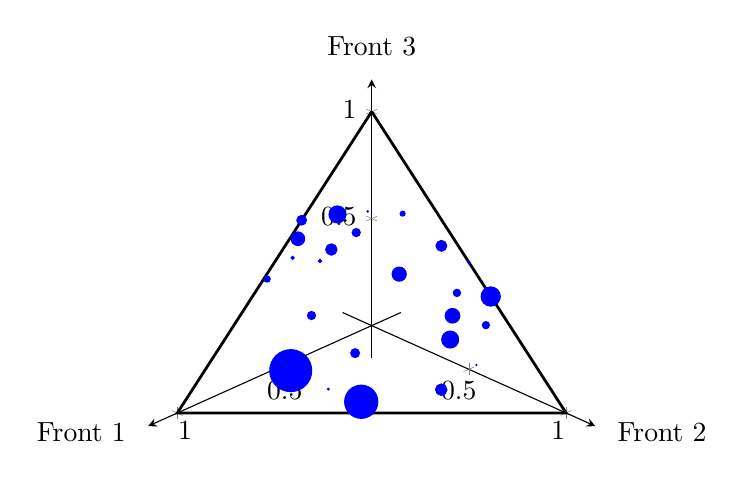
\begin{tikzpicture}
\begin{axis}[
    view={135}{30},
    xlabel={Front 1},
    ylabel={Front 2},
    zlabel={Front 3},
    xmin=0,
    xmax=1,
    ymin=0,
    ymax=1,
    zmin=0,
    zmax=1,
    width=8cm,
    height=8cm,
    axis lines=center,
    xlabel style={
        at={(ticklabel* cs:1.05)},
        anchor=east,
    },
    ylabel style={
        at={(ticklabel* cs:1.05)},
        anchor=west,
    },
    zlabel style={
        at={(ticklabel* cs:1.05)},
        anchor=south,
    },
    enlargelimits=0.15,
]
\addplot3[%
    scatter=true,
    only marks,
    mark=*,
    color=blue,
    point meta=explicit symbolic,
    scatter/@pre marker code/.style={/tikz/mark size=\pgfplotspointmeta*50},
    scatter/@post marker code/.style={}
] table[meta=w] {
x y z w
1.0 0.0 0.0 0.0
0.0 0.5 0.5 0.009654303207164589
0.25023023442966097 0.0 0.749769765570339 0.0
0.4932058353192057 0.18339681951996878 0.3233973451608256 0.029049980169382907
0.05650389511331322 0.8185970753584575 0.12489902952822926 0.0
0.41324231587781224 0.5867576841221878 0.0 0.0
0.6786405856065275 0.2903750381341887 0.03098437625928374 0.0
0.04349031055866048 0.4019373736382605 0.5545723158030791 0.038939095750905456
0.40076388878462343 0.021050456413010954 0.5781856548023656 0.04903090473416174
0.28243478105978426 0.6401915321648839 0.07737368677533185 0.04102671314930601
0.6648072334414368 0.0492306855836383 0.285962080974925 0.0
0.4814467233982045 0.5185532766017955 0.0 0.0
0.5468670648060134 0.00863406240441808 0.44449887278956846 0.022460565168244927
0.5862207793698717 0.39658897388822667 0.017190246741901616 0.0
0.17927649660562558 0.42246502397578034 0.39825847941859405 0.0
0.17632605612548735 0.5800034182869338 0.2436705255875789 0.06116312502553871
0.17595515345286916 0.15544262768706385 0.6686022188600669 0.004913497002613197
0.06062783145227446 0.6480035921955467 0.29136857635217883 0.02573772209026134
0.4434015332588057 0.3580189646073698 0.19857950213382447 0.0317522137806465
0.6505667816550538 0.1406871919800712 0.20874602636487505 0.0
0.0005920491605698741 0.6129137926298092 0.38649415820962096 0.0693668678563529
0.36046902825807403 0.0 0.639530971741926 0.03473597639610715
0.22308037099985156 0.27282562736959437 0.5040940016305541 0.0
0.13091929174218178 0.5465536126485865 0.3225270956092317 0.05273009731745313
0.3807376886206286 0.11485117054647198 0.5044111408328994 0.011743681147501262
0.5718755706169245 0.34901419767610814 0.0791102317069674 0.0059343257314523855
0.08158609957530605 0.5199658231548522 0.3984480772698417 0.02606561245934508
0.2523124234763152 0.5048769863677894 0.24281059015589534 0.0
0.2587178789380146 0.0824759880691166 0.6588061329928687 0.06115018279390709
0.31979246746766377 0.5397979595882282 0.14040957294410805 0.0
0.0897597760074555 0.2488346628453484 0.6614055611471962 0.017752319832239367
0.6033479577565064 0.29409578686799936 0.10255625537549427 0.0
0.4185724773649851 0.4447976227489905 0.13662989988602436 0.0
0.2405922803031214 0.160868318172387 0.5985394015244916 0.029275557559801872
0.1510666841314512 0.6895558742600341 0.1593774416085148 0.0034854601099706677
0.5082709727439931 0.4544398062393061 0.037289221016700735 0.1197678059454477
0.4460005375907148 0.03929476881514227 0.514704693594143 0.010953995589564676
0.3326427904764855 0.12496673516560852 0.542390474357906 0.04086140412689088
0.19889502688623395 0.34038407361247286 0.4607208995012932 0.0509852939350661
0.6379954308633884 0.2214620982069253 0.1405424709296862 0.15146329912067436
};
\addplot3[
    color=black,
    line width=1pt,
    mark=none,
] table {
x y z
0 0 1
0 1 0
1 0 0
0 0 1
};
\end{axis}
\end{tikzpicture}
\caption{The recovered strategy of Player 1 after 40 iterations drawn as points on a simplex with weight being indicated by their size. }
\label{fig:ex.blotto.slow.simplex}
\end{figure}
\end{example}

\begin{example}[Zero-sum polynomial game \cite{ParriloIEEE06}]\label{ex0}
    Consider a two-player zero-sum game with strategy sets $[-1,1]$ and a utility function of the first player
    \[
      u(x,y) = 2xy^2 - x^2 - y.
    \]

    As the generated subgames are all finite two-player zero-sum games, we can use linear programming to find their equilibria. The best response oracles were implemented using Lasserre's hierarchies.

    \begin{figure}
      \centering
      \label{figure0}
      
\includegraphics{do2.pdf}
      \caption{Convergence in Example \ref{ex0}. After 10 iterations, our method finds pure strategies $x \approx 0.4$ and $y \approx 0.63$, resulting in payoffs \((-0.47, 0.47)\). }
    \end{figure}
\end{example}

\begin{example}[General-sum polynomial game \cite{SteinOzdaglarParrilo08}]\label{ex1}
  The strategy set of each player is $[-1,1]$ and utility functions are
  \begin{align*}
    u_{1}(x,y) & = -3x^2y^2 - 2x^3 + 3y^3 + 2xy - x,\\
    u_{2}(x,y) &= 2x^2y^2 + x^2y - 4y^3 - x^2 + 4y.
  \end{align*}

  We computed equilibria in the general-sum matrix subgames using the multilinear program \ref{eq:sturmfels}. The best response oracles were implemented using Lasserre's hierarchies again.

  \begin{figure}
    \centering
    
\includegraphics{do3.pdf}
    \caption{Convergence in Example \ref{ex1}. Our method finds mixed strategies where $x\approx0.11$ with probability $44.19\%$ and $x\approx-1$ with probability $55.81\%$ and $y\approx0.72$ resulting in payoffs \((1.13, 1.81)\).}
  \end{figure}
\end{example}

\begin{example}[Torus game \cite{Chasnov20}]\label{ex2}
  Each strategy set is the unit circle $S^1 = [-\pi, \pi]$ and the utility functions are
  \begin{align*}
    u_{1}(\theta_1, \theta_2) &= \alpha_1 \cos(\theta_1 - \phi_1) - \cos(\theta_1 - \theta_2),\\
    u_{2}(\theta_1, \theta_2) &= \alpha_2 \cos(\theta_2 - \phi_2) - \cos(\theta_2 - \theta_1).
  \end{align*}
  parametrized by $\phi = (0, \pi/8)$ and $\alpha = (1, 1.5)$.

  We implemented the best response oracles using the spatial Branch and Bound method implemented by the \emph{Couenne} solver. We note that both the \emph{Gurobi} solver and \emph{SCIP} can also accept trigonometric functions as constraints. The general-sum master-problem was solved using the multilinear approach again.

  \begin{figure}
    \centering
    
\includegraphics[width=0.8\textwidth]{do1.pdf}
    \caption{Convergence in Example \ref{ex2}. We obtained pure strategies $\theta_1 \approx -1.06$, $\theta_2 \approx 1.01$ resulting in payoffs \((0.97, 1.71)\).}
  \end{figure}
\end{example}

\begin{example}[General Blotto \cite{Golman09}]\label{ex3}
  Each strategy set in this two-player zero-sum game is the standard $4$-dimensional simplex in $\R^5$ and the utility function of the first player is
  \[
    u(\textbf{x}, \textbf{y}) = \sum_{j=1}^5 f(x_j - y_j),
  \]
  where $f(x) = \sgn(x)\cdot x^2$.

  The master problem reduces to linear programming. We chose to implement the oracles using spatial Branch and Bound with symbolic reformulation (\cref{sec:sbab}) in \emph{Gurobi}. We modeled the $\sgn$ function using the following piecewise linear approximation:
  \[
    \sgn(x) \approx \begin{cases*}
      -1 & \text{if $x \le 0$}\\
      +1 & \text{otherwise}
    \end{cases*}.
  \]
  Since the multiplier $x^2$ will be zero, it is acceptable to ignore the behavior of this $\sgn$ approximation around zero.

  \begin{figure}
    \centering
    
\includegraphics[width=0.8\textwidth]{do6.pdf}
    \caption{Convergence in Example \ref{ex3}. We recovered pure strategies $\textbf{x} \approx (0, 0, 1, 0, 0)$ and $\textbf{y} \approx (1, 0, 0, 0, 0)$ resulting in payoffs \((0, 0)\). This is an~equilibrium computed by \textcite[Proposition 5]{Golman09}}
  \end{figure}
\end{example}


\begin{example}[Random polymatrix games]\label{exsep}
  Separable network games (polymatrix games) with finitely many strategies of each player can be solved in polynomial time \cite{Cai16} by linear programming. We use Algorithm \ref{alg:do} to compute equilibria of five-player polymatrix games defined by 20 by 20 matrices. Specifically, we generated a random matrix for each edge in the network and then transposed and subtracted the matrix of utility functions to make the game globally zero sum. We remark that zero-sum polymatrix games are payoff-equivalent to the general polymatrix games by \cite[Theorem 7]{Cai16}. In a test of 100 games, our algorithm found an $\eps$-equilibrium with $\eps = 0.01$ after $17.69$ iterations in a mean time of $0.29$ seconds.
\end{example}

\begin{example}[Three-player separable network game]\label{ex4}
  Further, we considered a continuous generalization of separable network games with strategy sets $[-1,1]$ and polynomial utility functions. This class of games was analyzed with the tools of polynomial optimization in \cite{KroVaVo}. There are 3 players. All pairs of players are involved in bilateral general-sum games and each player uses the same strategy across all such games. The pairwise utility functions are:
  \begin{equation*}
    \begin{aligned}
      u_{1, 2}(x_1,x_2) &= -2x_1x_2^2 + 5x_1x_2 - x_2\\
      u_{1, 3}(x_1,x_3) &= -2x_1^2 - 4x_1x_3 - 2x_3\\
      u_{2, 1}(x_2,x_1) &= 2x_1x_2^2 - 2x_1^2 - 5x_1x_2 + x_2\\
      u_{2, 3}(x_2,x_3) &= -2x_2x_3^2 - 2x_2^2 + 5x_2x_3\\
      u_{3, 1}(x_3,x_1) &= 4x_1^2 + 4x_1x_3 + 2x_3\\
      u_{3, 2}(x_3,x_2) &= 2x_2x_3^2 + 2x_2^2 - 5x_2x_3
    \end{aligned}
  \end{equation*}
  \begin{figure}
    \centering
    
\includegraphics{do7.pdf}
    \caption{Convergence in Example \ref{ex4}. Our method finds the mixed strategies where $x_1 \approx -0.06$, $x_2$ is $0.35$ with probability $0.708$ and $0.36$ with probability $0.292\%$, $x_3$ is $1.0$ with probability $0.7211$ and $-1.0$ with probability $0.2789$; with the corresponding payoffs \((-1.23, 0.26, 0.97)\).}
  \end{figure}
\end{example}


\section{Multiple Oracle Algorithm in Practice}


So far we focused on cases where the oracles and the master-problem would be tailored to each game individually. While this worked well, it raises the question of how applicable our technique is. In this section we will show that the branch and bound reformulations that were described in \cref{sec:sbab} can be successfully applied to solve a wide range of games, without the need to develop a new oracle each time. Similarly, given a sufficiently fast solver for finite general-sum games, it may be unnecessary to select more specific methods for solving the master-problem depending on the class of game. 

A consistent use of one particular master-problem and oracle method also allows us to finally measure and report meaningful run-times of the Multiple Oracle algorithm. For this reason, we compiled a test set of continuous games appearing in the game-theoretic and optimization-focused literature. The full list is in \cref{appendix:games} and covers 
games with polynomial, rational-polynomial, as well as generic utility functions, that are played over compact sets including intervals and simplexes, and whose equilibria are known to be pure, mixed, and even infinitely supported.

\subsection{Implementation}
blah... the following works well for us...

\paragraph{Initialization}
Blah... We initialize the algorithm by first selecting a feasible point in the interior of the players' strategy spaces and then allowing each player to select a best response to the feasible point. The algorithm then continues with standard Multiple Oracle iterations: by computing an equilibrium of the finite subgame and selecting additional best responses.

\paragraph{Nash Equilibria in Finite General-Sum Games}
Blah... While the \ref{eq:sturmfels} formulation worked acceptably well with \emph{Gurobi}, it appears that its performance relies on optimizations specific to the Baron solver, which we could not run extensive benchmarks on for practical reasons. Instead, we used the \emph{Gambit logit} utility, as it was the fastest and most reliable method for solving finite general-sum games in our testing.

\paragraph{Oracles}
Blah... The examples in our collections have utilities specified in terms of sums and products of functions such as logarithms and square roots. All such functions should be accepted either directly by global solvers or through external modeling libraries such as \textsc{ampl}.
\subsection{Results}
\input{chapter-continuous/quack-results.tex}

\end{document}
